\documentclass[12pt]{article}

\usepackage{sbc-template}

\usepackage{graphicx,url}

\usepackage[brazil]{babel}   
%\usepackage[latin1]{inputenc}  
\usepackage[utf8]{inputenc}  
% UTF-8 encoding is recommended by ShareLaTex

\usepackage{indentfirst}
     
\sloppy

\title{SISACS - Sistema de auxílio comunitário de saúde}

\author{Alberto Zaranza Valença de Freitas\inst{1}, Joel da Silva Uchoa\inst{1}}

\address{Instituto Federal de Educação, Ciência e Tecnologia do Ceará - Campus Aracati (IFCE)\\
  Rodovia CE-040, Km 137,1, s/n - Aeroporto, Aracati - CE, 62800-000
  \email{albertozaranza@gmail.com, joeluchoa@ifce.edu.br}
}

\begin{document} 

\maketitle

\begin{abstract}
    This article aims to explain the advantages of using the mobile application developed to streamline the process of home visits of community health agents in the city of Aracati-CE, as well as to optimize the work of typists who feed the e-SUS.
\end{abstract}
     
\begin{resumo} 
  Este artigo tem o objetivo de explanar as vantagens de utilizar a aplicação para dispositivos móveis desenvolvida para tornar mais ágil o processo de visitas domiciliares de agentes comunitários de saúde da cidade de Aracati-CE, além de otimizar o trabalho de digitadores que alimentam o sistema do e-SUS.
\end{resumo}


\section{Introdução}

As tecnologias móveis vêm causando mudanças significativas na sociedade. Isso se tornou possível graças ao acesso de qualquer tipo de informação na palma da mão, por meio de celulares ou tablets, mais especificamente, as tecnologias móveis. Entretanto, nem sempre foi assim, tudo começou na época que foram inventados os aparelhos celulares, entre as décadas de 1940 e 1950. Eles eram apenas capazes de realizar ligações através de ondas eletromagnéticas que permitiam a transmissão bidirecional de voz e dados utilizáveis em uma área geográfica que se encontra dividida em células (de onde provém a nomenclatura celular), cada uma delas servida por um transmissor/receptor. Com o decorrer dos anos, foram adicionadas novas aplicabilidades aos dispositivos, dentre elas: envio de mensagens através do SMS (\textit{Short Message Service} - em português: serviço de mensagens curtas), programação de alarmes para despertar uma pessoa, gravação de lembretes, possibilidade de tirar fotos e gravar vídeos,  jogar, ouvir música, usar sistemas de posicionamento global para localização, dentre outras. Com tantas funções implementadas em um curto período de tempo (cerca de uma década e meia), esses aparelhos começaram a ser chamados de \textit{smartphones}.

A partir desse momento foi notado o quão importante esses aparelhos poderiam ser, não apenas para o entretenimento, mas também para o monitoramento da sua saúde corporal com a ajuda de \textit{gadgets}, equipamentos criados para facilitar funções específicas e úteis no cotidiano, tais como monitoramento de batimentos cardíacos, cálculos de IMC (índice de massa corporal), além de também poderem ser usados para o beneficio de uma comunidade.

Em se tratando de saúde pública no Brasil, é possível perceber que a mesma passa por imensas dificuldades no país, desde a superlotação de hospitais, faltas de médicos, à aplicação incorreta de recursos. Em postos de saúde não é muito diferente, entretanto, além de demandas da comunidade por atendimentos e remédios, eles têm que lidar com grande quantidade de informações que necessitam ser enviadas para o governo federal, dados esses, que são coletados por agentes comunitários de saúde em visitas domiciliares e territoriais através de formulários de papel, onde todos os dados são manuscritos, e em seguida são repassadas para o sistema do e-SUS através dos digitadores.
Todavia, fichas dos mais variados tipos, acabam ficando empilhadas para serem digitadas apenas por um funcionário, podendo ocasionar também erros de digitação.  Logo, é de extrema importância que esse processo seja agilizado para não sofrer com falta de recursos provenientes das administrações superiores.

Analisando todo esse cenário, surge a ideia de usar as tecnologias disponíveis para a criação de uma aplicação para dispositivos móveis que auxilie agentes comunitários de saúde em visitas domiciliares e territoriais de forma a ser fazer dispensável o uso de fichas de papel e tornar esse processo mais ágil.

\section{First Page} \label{sec:firstpage}

The first page must display the paper title, the name and address of the
authors, the abstract in English and ``resumo'' in Portuguese (``resumos'' are
required only for papers written in Portuguese). The title must be centered
over the whole page, in 16 point boldface font and with 12 points of space
before itself. Author names must be centered in 12 point font, bold, all of
them disposed in the same line, separated by commas and with 12 points of
space after the title. Addresses must be centered in 12 point font, also with
12 points of space after the authors' names. E-mail addresses should be
written using font Courier New, 10 point nominal size, with 6 points of space
before and 6 points of space after.

The abstract and ``resumo'' (if is the case) must be in 12 point Times font,
indented 0.8cm on both sides. The word \textbf{Abstract} and \textbf{Resumo},
should be written in boldface and must precede the text.

\section{CD-ROMs and Printed Proceedings}

In some conferences, the papers are published on CD-ROM while only the
abstract is published in the printed Proceedings. In this case, authors are
invited to prepare two final versions of the paper. One, complete, to be
published on the CD and the other, containing only the first page, with
abstract and ``resumo'' (for papers in Portuguese).

\section{Sections and Paragraphs}

Section titles must be in boldface, 13pt, flush left. There should be an extra
12 pt of space before each title. Section numbering is optional. The first
paragraph of each section should not be indented, while the first lines of
subsequent paragraphs should be indented by 1.27 cm.

\subsection{Subsections}

The subsection titles must be in boldface, 12pt, flush left.

\section{Figures and Captions}\label{sec:figs}


Figure and table captions should be centered if less than one line
(Figure~\ref{fig:exampleFig1}), otherwise justified and indented by 0.8cm on
both margins, as shown in Figure~\ref{fig:exampleFig2}. The caption font must
be Helvetica, 10 point, boldface, with 6 points of space before and after each
caption.

\begin{figure}[ht]
\centering
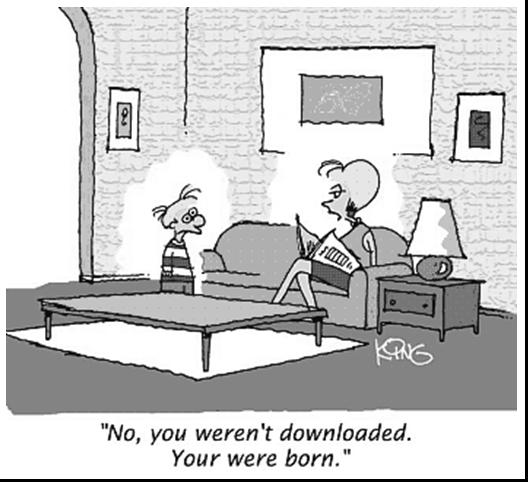
\includegraphics[width=.5\textwidth]{fig1.jpg}
\caption{A typical figure}
\label{fig:exampleFig1}
\end{figure}

\begin{figure}[ht]
\centering
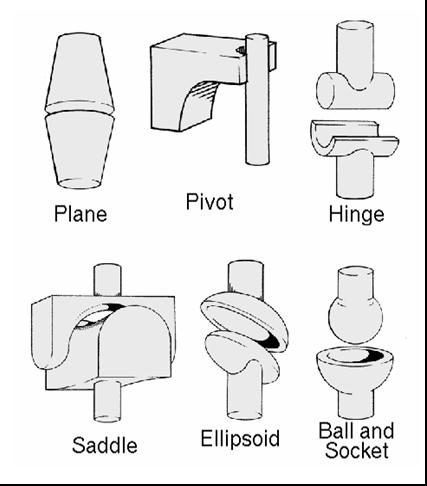
\includegraphics[width=.3\textwidth]{fig2.jpg}
\caption{This figure is an example of a figure caption taking more than one
  line and justified considering margins mentioned in Section~\ref{sec:figs}.}
\label{fig:exampleFig2}
\end{figure}

In tables, try to avoid the use of colored or shaded backgrounds, and avoid
thick, doubled, or unnecessary framing lines. When reporting empirical data,
do not use more decimal digits than warranted by their precision and
reproducibility. Table caption must be placed before the table (see Table 1)
and the font used must also be Helvetica, 10 point, boldface, with 6 points of
space before and after each caption.

\begin{table}[ht]
\centering
\caption{Variables to be considered on the evaluation of interaction
  techniques}
\label{tab:exTable1}
\smallskip
\begin{tabular}{|l|c|c|}
\hline
& Value 1 & Value 2\\[0.5ex]
\hline
&&\\[-2ex]
Case 1 & 1.0 $\pm$ 0.1 & 1.75$\times$10$^{-5}$ $\pm$ 5$\times$10$^{-7}$\\[0.5ex]
\hline
&&\\[-2ex]
Case 2 & 0.003(1) & 100.0\\[0.5ex]
\hline
\end{tabular}
\end{table}

\section{Images}

All images and illustrations should be in black-and-white, or gray tones,
excepting for the papers that will be electronically available (on CD-ROMs,
internet, etc.). The image resolution on paper should be about 600 dpi for
black-and-white images, and 150-300 dpi for grayscale images.  Do not include
images with excessive resolution, as they may take hours to print, without any
visible difference in the result. 

\section{References}

Bibliographic references must be unambiguous and uniform.  We recommend giving
the author names references in brackets, e.g. \cite{knuth:84},
\cite{boulic:91}, and \cite{smith:99}.

The references must be listed using 12 point font size, with 6 points of space
before each reference. The first line of each reference should not be
indented, while the subsequent should be indented by 0.5 cm.

\bibliographystyle{sbc}
\bibliography{sbc-template}

\end{document}
